%% This is an example first chapter.  You should put chapter/appendix that you
%% write into a separate file, and add a line \include{yourfilename} to
%% main.tex, where `yourfilename.tex' is the name of the chapter/appendix file.
%% You can process specific files by typing their names in at the 
%% \files=
%% prompt when you run the file main.tex through LaTeX.
\chapter{Reconstructed Objects}

The state-of-the-art CMS detector take a snapshot of each event and saves the detailed information of the collisions into datasets. In the datasets, we can access to event information with fully reconstructed objects including hits, tracks, muons, and vertex, which will be crucial for our data analysis to study B meson physics in heavy-ion collisions. Below, we will describe, in principle, how these objects with physical meaning are reconstructed from electronic signal in the CMS detector.

\section{Event}

As mentioned previously, an event is defined as a snapshot of one collision at the LHC. Many particles are produced in the collisions and then decay before they are detected in an event. Theoretically, to obtain the complete information of an event, we only need to know the position and momentum of each particle. Experimentally, we detect final state particles and record their kinematics. In high energy physics experiments, the particles reaching the detectors are $e^{\pm}$, $\mu^{\pm}$, $\pi^{\pm}$, $K^{\pm}$, $p$, $n$, $K^0_L$, $\gamma$. All other particles already decayed into these particles before they can be detected. In order to study them, they need to be reconstructed. Historically, this is used to be done by fast camera with high resolution. The Figure \ref{OmegaNick} shows a famous $\Omega^-$ baryon (Strangeness -3: $sss$) event reconstructed from one of picture taken in the bubble chamber \cite{OmegaNick}.

\begin{figure}[hbtp]
\begin{center}
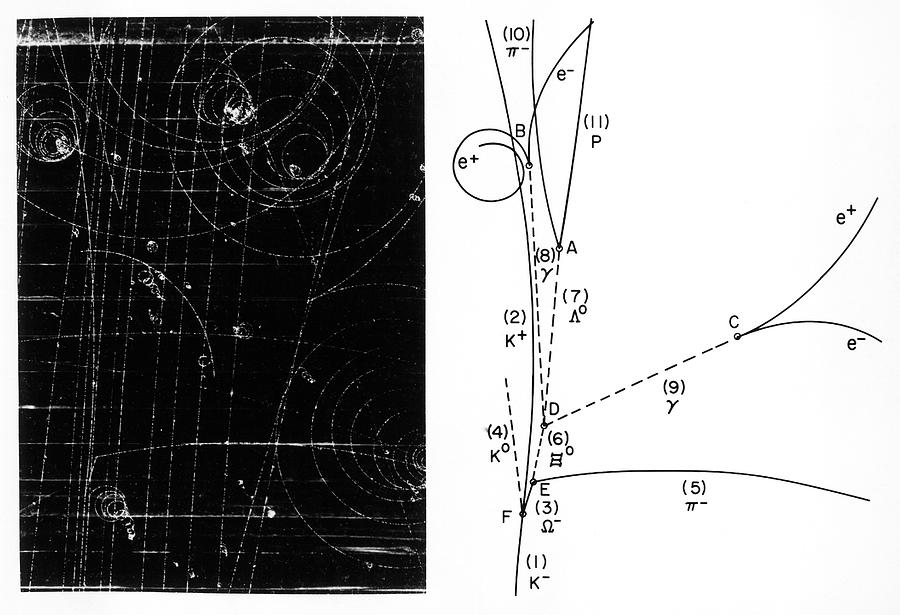
\includegraphics[width=0.70\textwidth]{Figures/Chapter3/Omega.jpg}
\caption{The bubble chamber picture of the an $\Omega^-$ baryon reconstructed from an event: $K^- p \rightarrow K^0 K^+ \Omega^- \rightarrow \Xi^0 \pi^- \rightarrow \Lambda^0 \gamma \gamma \rightarrow \pi^- p$ taken from the group led by Nicholas Samios at BNL is shown above.}
\label{OmegaNick}
\end{center}
\end{figure} 


Nowadays, the technologies have advanced. With the development of computing, detector hardware and readout electronics, high energy physics experiments are able to collect many events with higher precision of measurements. For instance, the CMS experiment has an event trigger rate of 100kHz, which corresponds to a rate of 100000 events per second with 100 GB/s information \cite{CMSDAQ}. Experimental data have become more digital and abstract instead of pictorial and intuitive. All events information is stored at a file format instead of a photograph. Physicists use computer to read the experimental data and develop software to perform analysis of each event, extract the physics information from the analysis, and interpret the physics results. 

In the following subsections, for simplicity, I will explain the reconstructed objects of events with only one charged particle. 

\section{Hit}

All reconstructed objects start from hits as the energy deposition of particle passing through the detectors. Here I will explain the concept of hits based on CMS silicon pixel tracker. Figure \ref{CMSPixChip}, the schematic view of a chip with silicon pixels in the CMS tracker


\begin{figure}[hbtp]
\begin{center}
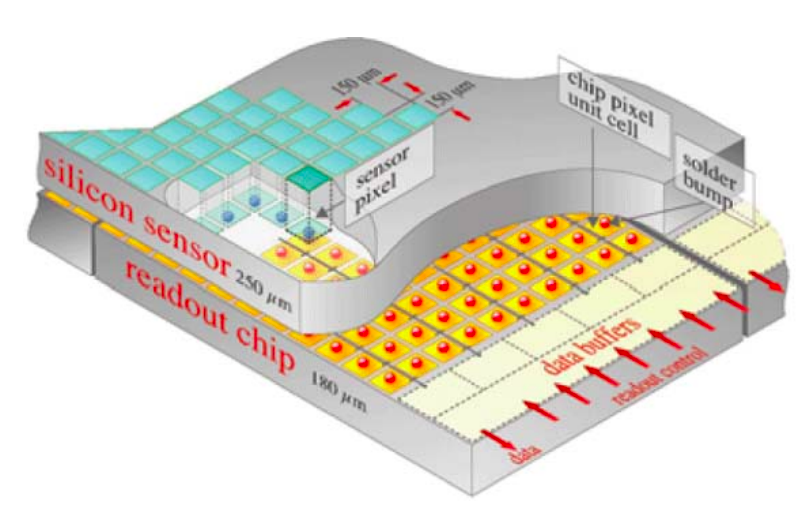
\includegraphics[width=0.50\textwidth]{Figures/Chapter3/CMSPixChip.png}
\caption{The schematic plot of a CMS silicon chip with pixel sensor is shown above.}
\label{CMSPixChip}
\end{center}
\end{figure} 

When a charged particle pass through a layer of the CMS silicon pixel detector, we can look at the charges collected by each pixel on that layer due to the ionization of electron-hole pairs by the high energy charged particle. Ideally, if a particle enter the tracker at a normal angle, only one pixel is fired. However, in reality, its neighboring pixels may also have some response. When the particle enter the tracker with a small angle  particularly when the part. Figure \ref{HitDemo} schematically demonstrates the firing pixel when a particle passing the layer

\begin{figure}[hbtp]
\begin{center}
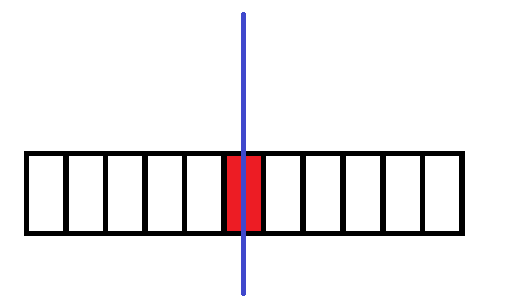
\includegraphics[width=0.48\textwidth]{Figures/Chapter3/Hit1.png}
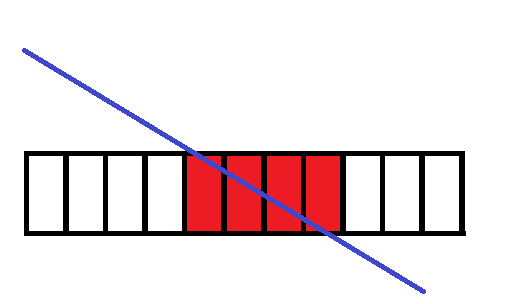
\includegraphics[width=0.48\textwidth]{Figures/Chapter3/Hit2.png}
\caption{The schematic views of a charged particle (blue line) entering the silicon pixel layer (black) at a normal angle (left) and a small tilting angle (right) with the pixels fired (red) are shown above. The left cluster has 1 hit and the right cluster has 4 hits.}
\label{HitDemo}
\end{center}
\end{figure} 

Here we call each firing pixel as a hit, which is demonstrated above in Figure \ref{HitDemo} in red. In CMS pixel tracker, the probability of a pixel firing when a charged particle passing through is greater than 99\% \cite{CMSTrackComp}, which means that it is very unlikely a hit is missing when a particle pass through the pixel. 



\section{Cluster}

Therefore, there should be at least one hit for each layer when a single particle pass through. We call the collection of the adjacent pixel hits in a layer due to one particle as a cluster \cite{CMSTrackComp}. The number of electric charges $Q$ is associated to each hit. We can design an algorithm determine the center of a cluster according to the charges of each hit. A simple algorithm is to calculate the center of gravity of the cluster taking the weighted averaging of the charge and the position of each hit. In this case, for a cluster with a single hit, its position is simply the center of the pixel. For clusters with many hits, we develop a dedicated algorithm to estimate its position \cite{CMSTrackComp}. The position of a cluster is a measurement of the particle trajectory. 

However, in an event with many particles, the occupancy of each layer will be busy and the clusters will become complicated. The CMS collaboration develop  In CMS terminology, the conversion of electronic signal of pixels to clusters is called DIGI.


\section{Tracklet}

In a uniform external magnetic field, the trajectory of a charged particle will be a helix in 3 dimensions. Geometrically, five parameters are needed to parametrize a helix. A parametric curve of a helix moving in the Cartesian coordinates moving in the z direction is written as follows

\begin{equation}
x(t) = R \cos(\omega t) + a
\end{equation}

\begin{equation}
y(t) = R \sin(\omega t) + b
\end{equation}

\begin{equation}
z(t) = v t + c
\end{equation}

Therefore, we need at least 3 clusters to determine the all 5 parameters. 3 clusters can determine the radius $R$ and the center of the circle (a,b) and also can determine the straight line in the z-direction. Figure \ref{HelixAndFit} shows the helix path of a charged particle in a uniform magnetic field and the fit to determine the center and the radius of the helix.


\begin{figure}[hbtp]
\begin{center}
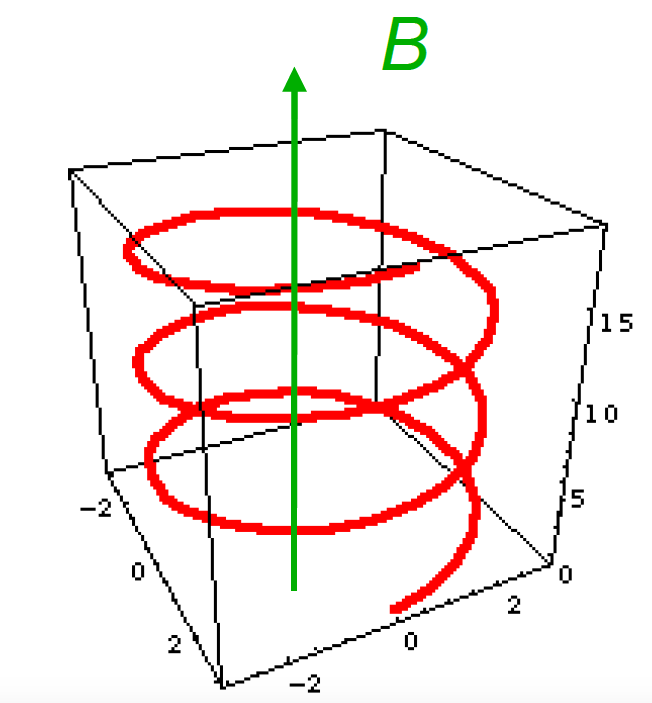
\includegraphics[width=0.35\textwidth]{Figures/Chapter3/Helix.png}
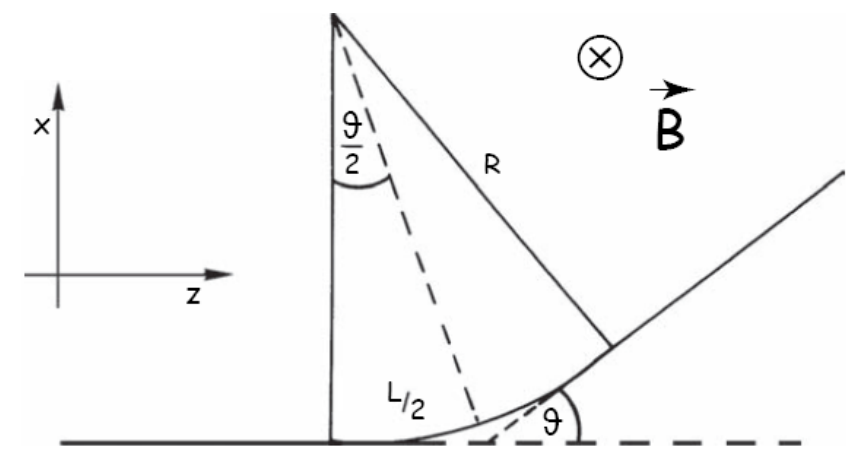
\includegraphics[width=0.55\textwidth]{Figures/Chapter3/FitToCircle.png}
\caption{The helix motion of a charged particle under a constant and uniform magnetic field $\vec{B}$ pointing in the +z direction (left) and the fit to 3 points to determine the center and the radius of a circle (right) are shown above.}
\label{HelixAndFit}
\end{center}
\end{figure} 

Moreover, we can determine transverse momentum of the charged particle according to the $R$ fitted from fit to the center of 3 clusters.

\begin{equation}
p_T  = qRB
\end{equation}

In general, the charges of the particles produced in the collision and pass through the tracker are $q = e$. Hence, $p_T = eRB$. For $p_T$ in the unit of GeV, $R$ in the unit of meter (m), and $B$ in the unit of tesla (T), we have 

\begin{equation}
p_T  \simeq 0.3 RB
\end{equation}

Therefore, as seen above from Figure \ref{HelixAndFit}, the transverse momentum resolution is driven by the determination of $R$ assuming we have a perfect measurement on the magnetic field $B$.

\begin{figure}[hbtp]
\begin{center}
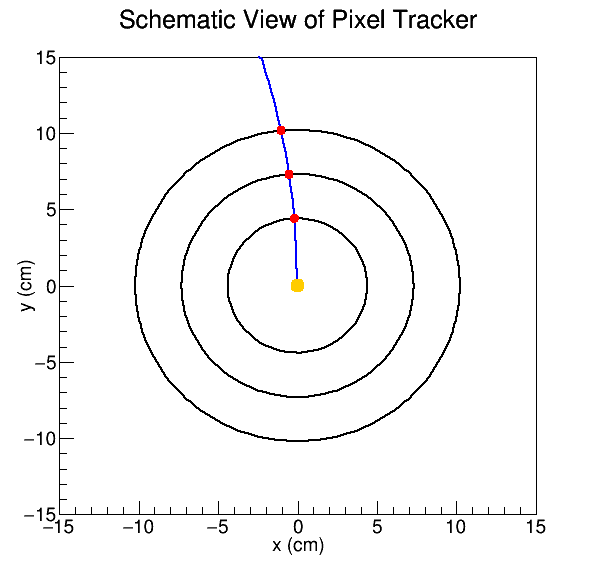
\includegraphics[width=0.45\textwidth]{Figures/Chapter3/PixLayTrk.png}
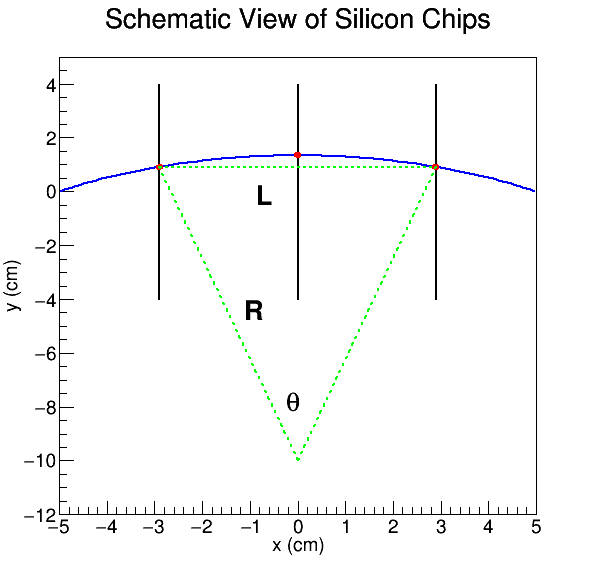
\includegraphics[width=0.45\textwidth]{Figures/Chapter3/FitOnHits.png}
\caption{A track (blue) initiated from the primary vertex (orange) passing through 3 layers of pixel detectors (black) with 3 clusters (red) is shown on the left and the circular fit to the 3 clusters with the definition of $R$, $L$, and $\theta$ is shown on the right.}
\label{HelixAndFit}
\end{center}
\end{figure} 



According to Figure \ref{HelixAndFit} on the right, at high $p_T$, essentially in parallel, for a 3 cluster fit. In addition, we know that the layers in the pixel track has equal spacing $\Delta r$ between layers. For CMS pixel tracker, its inner most 3 layers has equal distance $\Delta r_{12} = \Delta_{23} =$ 2.9 cm \cite{CMSPIXInfo}. 


Hence, we can see that $L/2 = \Delta r$, which assume fixed with no uncertainties. Hence, we have

\begin{equation}
\frac{L}{2} = R \sin \frac{\theta}{2}
\end{equation}

Again, at high $p_T$, the angle $\theta$ will be very small since the radius of the circle $R >> \Delta r$, $\sin\theta \simeq \theta$ and $\cos\theta \simeq 1 - \frac{\theta^2}{2}$. Hence, we can use small angle approximation

\begin{equation}
L = 2 R \sin \frac{\theta}{2} \simeq R \theta
\end{equation}

Therefore,

\begin{equation}
p_T  \simeq 0.3 RB = 0.3 \frac{BL}{\theta}
\end{equation}


Hence, geometrically, we have


\begin{equation}
s = R - R \cos \frac{\theta}{2} = R (1 -  \cos \frac{\theta}{2}) =  R (1 -  \cos \frac{\theta}{2})  \simeq  \frac{L}{\theta} \{1 - [1 - \frac{1}{2} (\frac{\theta}{2})^2] \} =  \frac{L\theta}{8} = \frac{0.3BL^2}{8p_T}
\end{equation}

Thus, the uncertainties on both sides go as 

\begin{equation}
\sigma_s =  \frac{0.3BL^2}{8p_T^2} \sigma_{p_T}
\end{equation}

Hence, the transverse momentum resolution $\frac{\sigma_{p_T}}{p_T}$ is given by 


\begin{equation}
\frac{\sigma_{p_T}}{p_T} = \frac{8\sigma_s}{0.3BL^2} p_T
\end{equation}

Here, $\sigma_s$ is effective the position resolution of the silicon pixel detector. We can see that the transverse momentum resolution gets worse as $p_T$ increases in the high $p_T$ region. Figure \ref{CMSpTReso} shows the $\frac{\sigma_{p_T}}{p_T}$ as a function $p_T$


\begin{figure}[hbtp]
\begin{center}
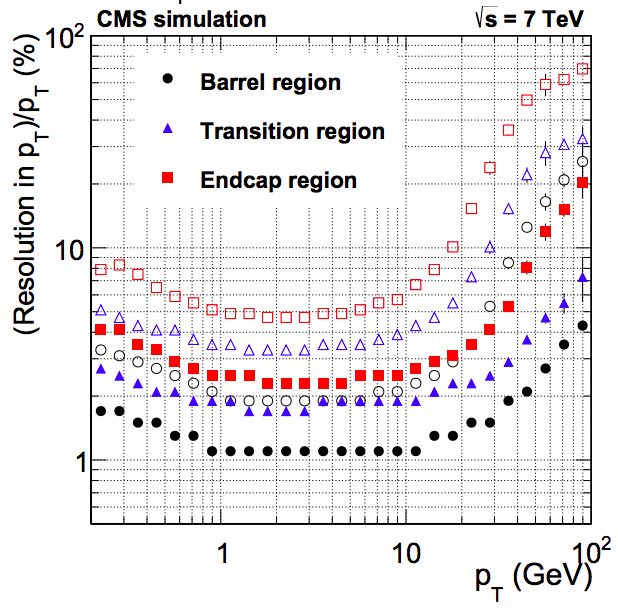
\includegraphics[width=0.60\textwidth]{Figures/Chapter3/CMSpTReso.png}
\caption{The transverse momentum resolution $\frac{\sigma_{p_T}}{p_T}$ of a track as a function of transverse momentum $p_T$ is shown above.}
\label{CMSpTReso}
\end{center}
\end{figure} 

We can see that a good agreement with linear growth of $\frac{\sigma_{p_T}}{p_T}$ for $p_T > 20$ GeV/c in the high $p_T$ region.

Longitudinally, $p_z$ can be determined by the $p_T$ and the angle $\Delta \theta$ in the transverse direction 

\begin{equation}
p_z = \frac{\Delta z}{\frac{R\Delta \theta}{p_T}} = 0.3B \frac{\Delta z}{\Delta \theta}
\end{equation}

Because the CMS silicon tracker has 3 pixel and 10 strip layers, a charge particle passing through all 13 layers should leave 13 clusters, which is much more than required to determine the helix. A dedicated seeding algorithm is designed to select the clusters and perform best fitting \cite{CMSTrackComp}. In addition, an iterative process to improve the fit and reduce fake track is implemented. Then, we can perform fits on these seeds. The fits to these seeds are called ``tracklets''.   
 

\section{Track}

With trackets from the seeds, we can reconstruct the tracks by the extending the tracklets \cite{Track}


After these process, we have reconstructed the objected from all the tracklets named a track



\section{Muon}




\section{Vertex}

\subsection{Primary Vertex}

\subsection{Secondary Vertex}

\section{Experimental Results}


Nevertheless, here I just take a simple case that only one charged particle is present in an event. In reality, LHC collision events in general have high pile with high multiplicity \cite{}. Figure \ref{} shows the number of reconstructed vertices in $pp$ collisions from MC and data. 


Therefore, when there are so many particles coming from many vertices in each event, the CMS Collaboration have designed more complicated algorithms to reconstruct events with physics objects mentioned above \cite{}.



